\section{SDN-based Dynamic Routing}
\subsection*{Dynamic Routing}
    Experiment 3에서 진행해본 Dynamic routing 알고리즘은 Shortest Path Algorithm 으로 이용하여 라우터가 최적의 경로를 찾는 방법으로 path를 결정해 준다. Experiment 2에서 Static Routing을 실험한것과 동일한  week7.py topology에서, proactive 방식으로 Dynamic routing을 구현하기 위해서 Pox controller애서 topo\_proactive.py라는 shortest path routing을 실행해 주었다.\\
    \vspace{-4mm}
    \begin{figure}[!h]\centering 
    	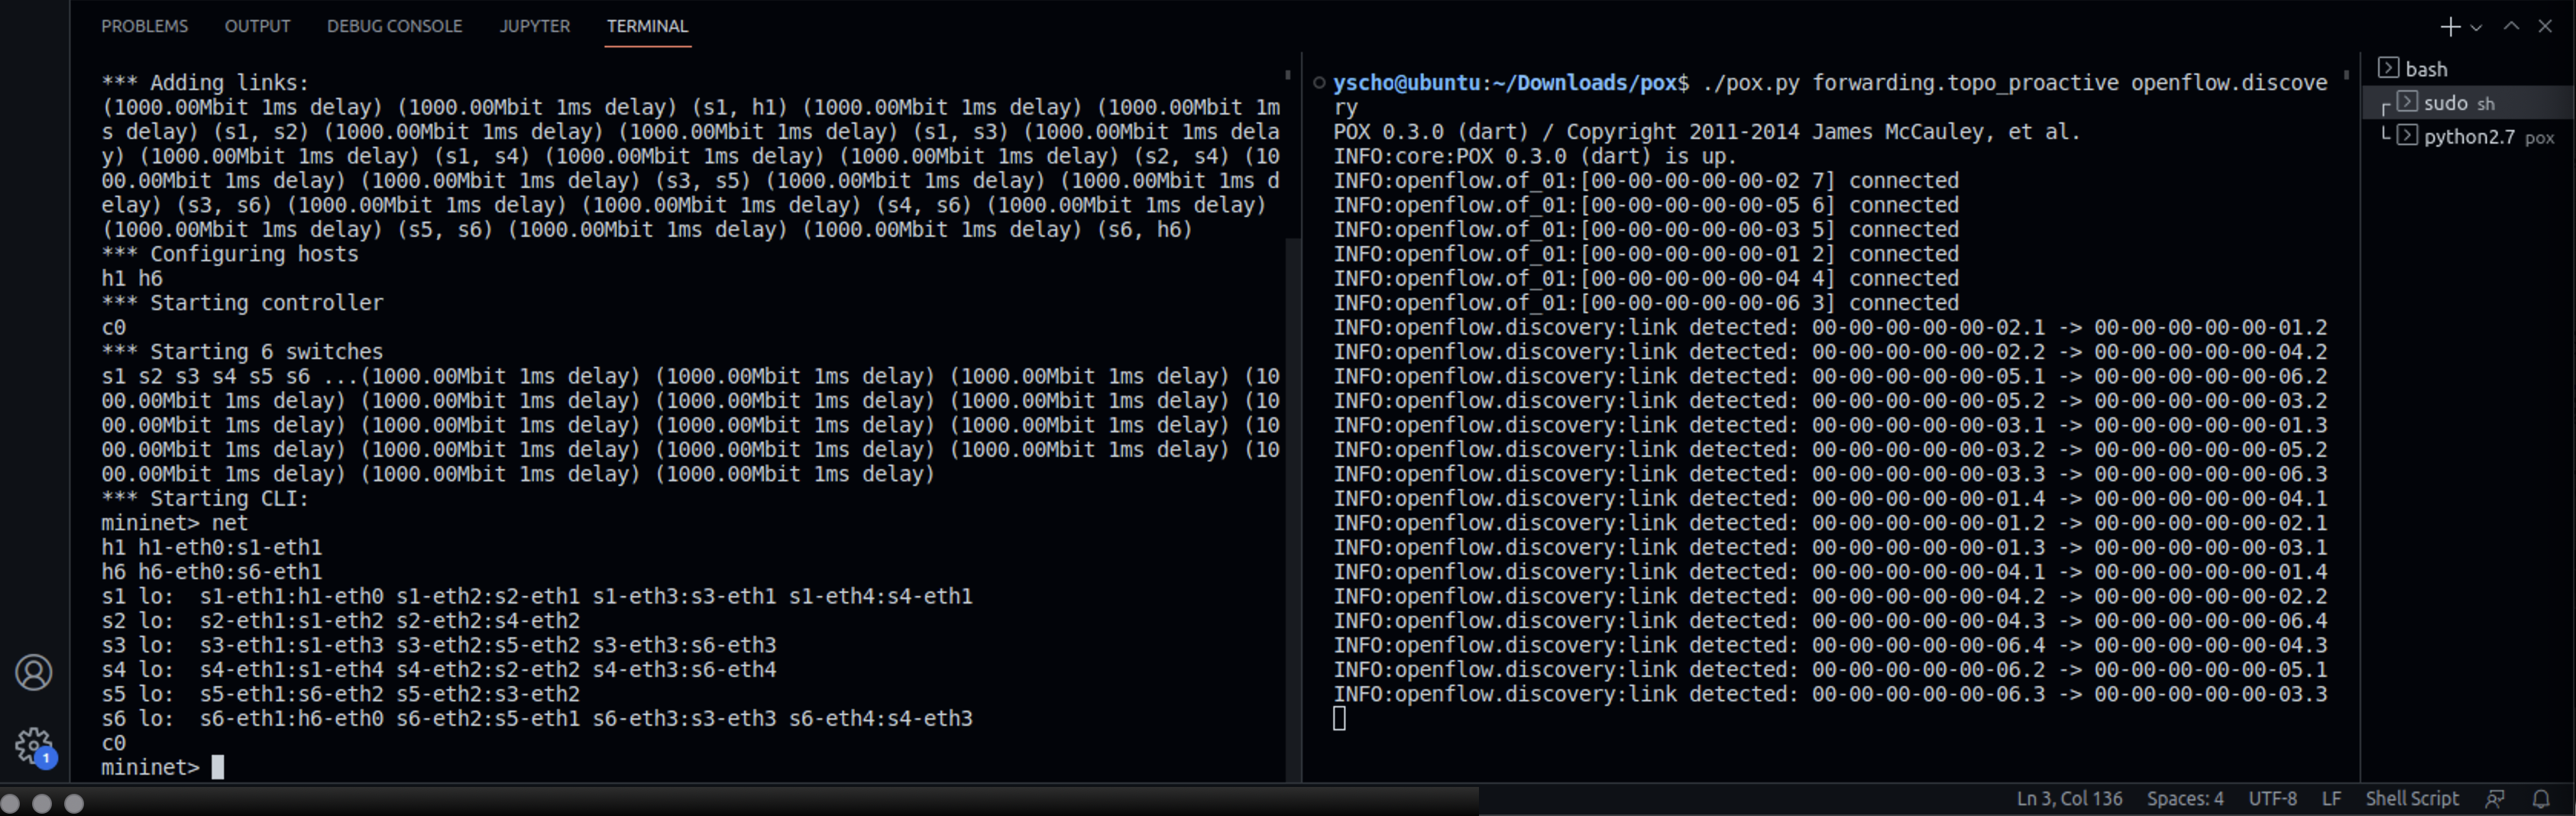
\includegraphics[width=.99\textwidth]{image/week08/3-0.png}
    	\caption{\footnotesize
    	 topo\_proactive.py 실행과 week07.py topo 실행후 discovery의 path의 결과를 확인할 수 있다.}
    	\vspace{-10pt}
    \end{figure}
        \vspace{-2mm}
    \subsection*{Flow Table}
    구성해준 환경에서 openflow swithch의 packet흐름을 확인하기 위해서 ‘datapath control’ command의 dump-flows 를 실행해 flow table을 출력해 주었다.\footnote{다음 페이지에 첨부}
        \subsubsection*{Flow Table Analysis}
        Flow Table에서 Flow는 packet을 전달하는 규칙이다. 즉 MAC address가 어떨때 openflow switch 내부에서 out을 어떤지 결정해주는 state이다. 다음의 flow table에서 input 조건에 따른 port 연결을 확인할 수 있다. switch 1번의 flow table을 예시로 확인해 보자.\\
        \vspace{-4mm}
        \begin{figure}[!h]\centering 
        	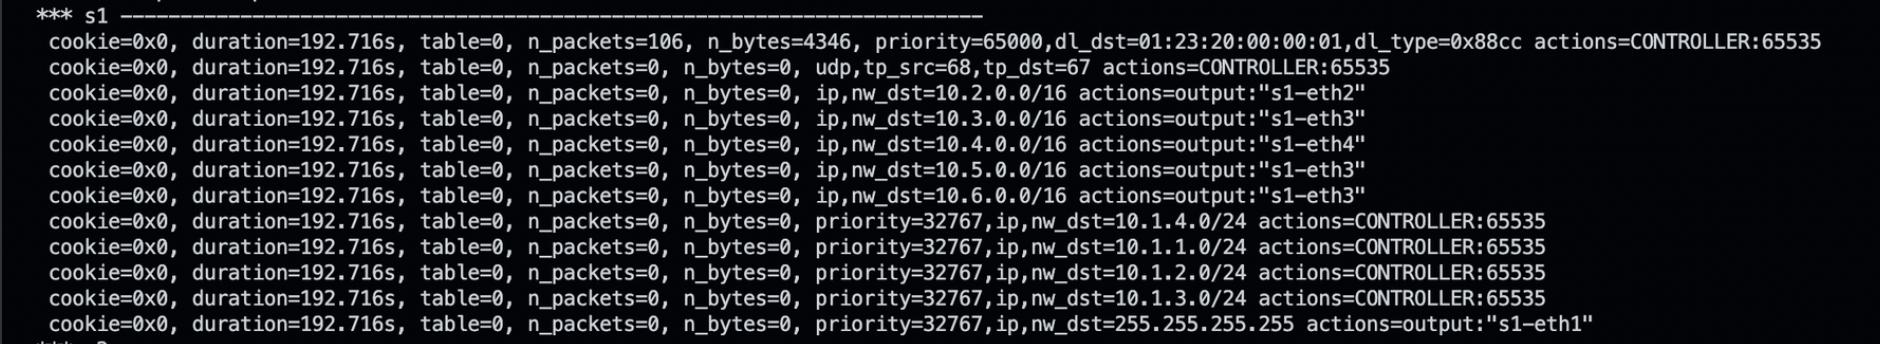
\includegraphics[width=.99\textwidth]{image/week08/3-1-1-1.png}
        	\caption{\footnotesize
        	  Switch 1 의 flow table}
        	\vspace{-10pt}
        \end{figure}
        
        Flow를 이루는 state에서 Switch 1번에서 전송되는 packet에서 가질 수 있는 destination 의 MAC address 는 10.6.0.0 또는 10.1.0,0을 가질 수 있다. flow table을 확인해 보면 dst 가 10.6.0.0일때 3번 포트 host와 연결된 MAC address가 10.1.0.0 일때 1번 포트임을 확인할 수 있다. 즉 path를 확인해 보기 위해서 실험 2-2에서 추가해준 data path control command와 비교해 주었다.  
        \clearpage
%---------------------------------------------------------------------------------%
        \begin{listing}[h!]
        \inputminted[framerule = 1pt,framesep = 2mm , frame = lines, fontsize=\footnotesize]{python}{./code/week08/flow2-2.sh}
        \vspace{-2mm}
        \caption{\footnotesize Experiment 2-2's dpctl flow-add commandss}
        \end{listing}
        
        switch 1 은 마찬가지로 Switch 3와 연결된 3번 포트와 연결된것을 확인할 수 있고, 마찬가지로 Switch 3에서도 Switch 6와 연결하기 위해서 s6과 연결된 포트 3번으로 flow가 작성된것을 확인할 수 있다. 따라서 proactive 알고리즘을 통해서 생성된 flow table의 path는 experiment 2-2에서 만들어준 static routing의 path와 동일함을 확인할 수 있다.\\
        \vspace{-4mm}
        \begin{figure}[!h]\centering 
        	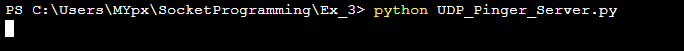
\includegraphics[width=.99\textwidth]{image/week08/3-1.png}
        	\caption{\footnotesize
        	  Experiment 3' flow table}
        	\vspace{-10pt}
        \end{figure}
            
        Dynamic Routing을 사용하는 SDN controller의 경로가  experiment 2-2의 path와 동이란지 Ping Test로 RTT를 측정함으로서 확인해 보자.
        \clearpage
%---------------------------------------------------------------------------------%
    \subsection*{Ping Test}
    1000개의 packet을 0.01 의 interval을 가지고 전송해주는 pingtest 결과 Experiment 2-2 의 average RTT인 \textbf{$10.261\ ms$}에 근사한 \textbf{$10.331\ ms$}이 측정되었다. 따라서 Dynamic Routing의 shortest path algorithm을 적용한 path는 Expeiment 2-2와 동일한 path를 통해서 routing이 이루어짐을 확인할 수 있었다.\\
    \vspace{-4mm}
    \begin{figure}[!h]\centering 
    	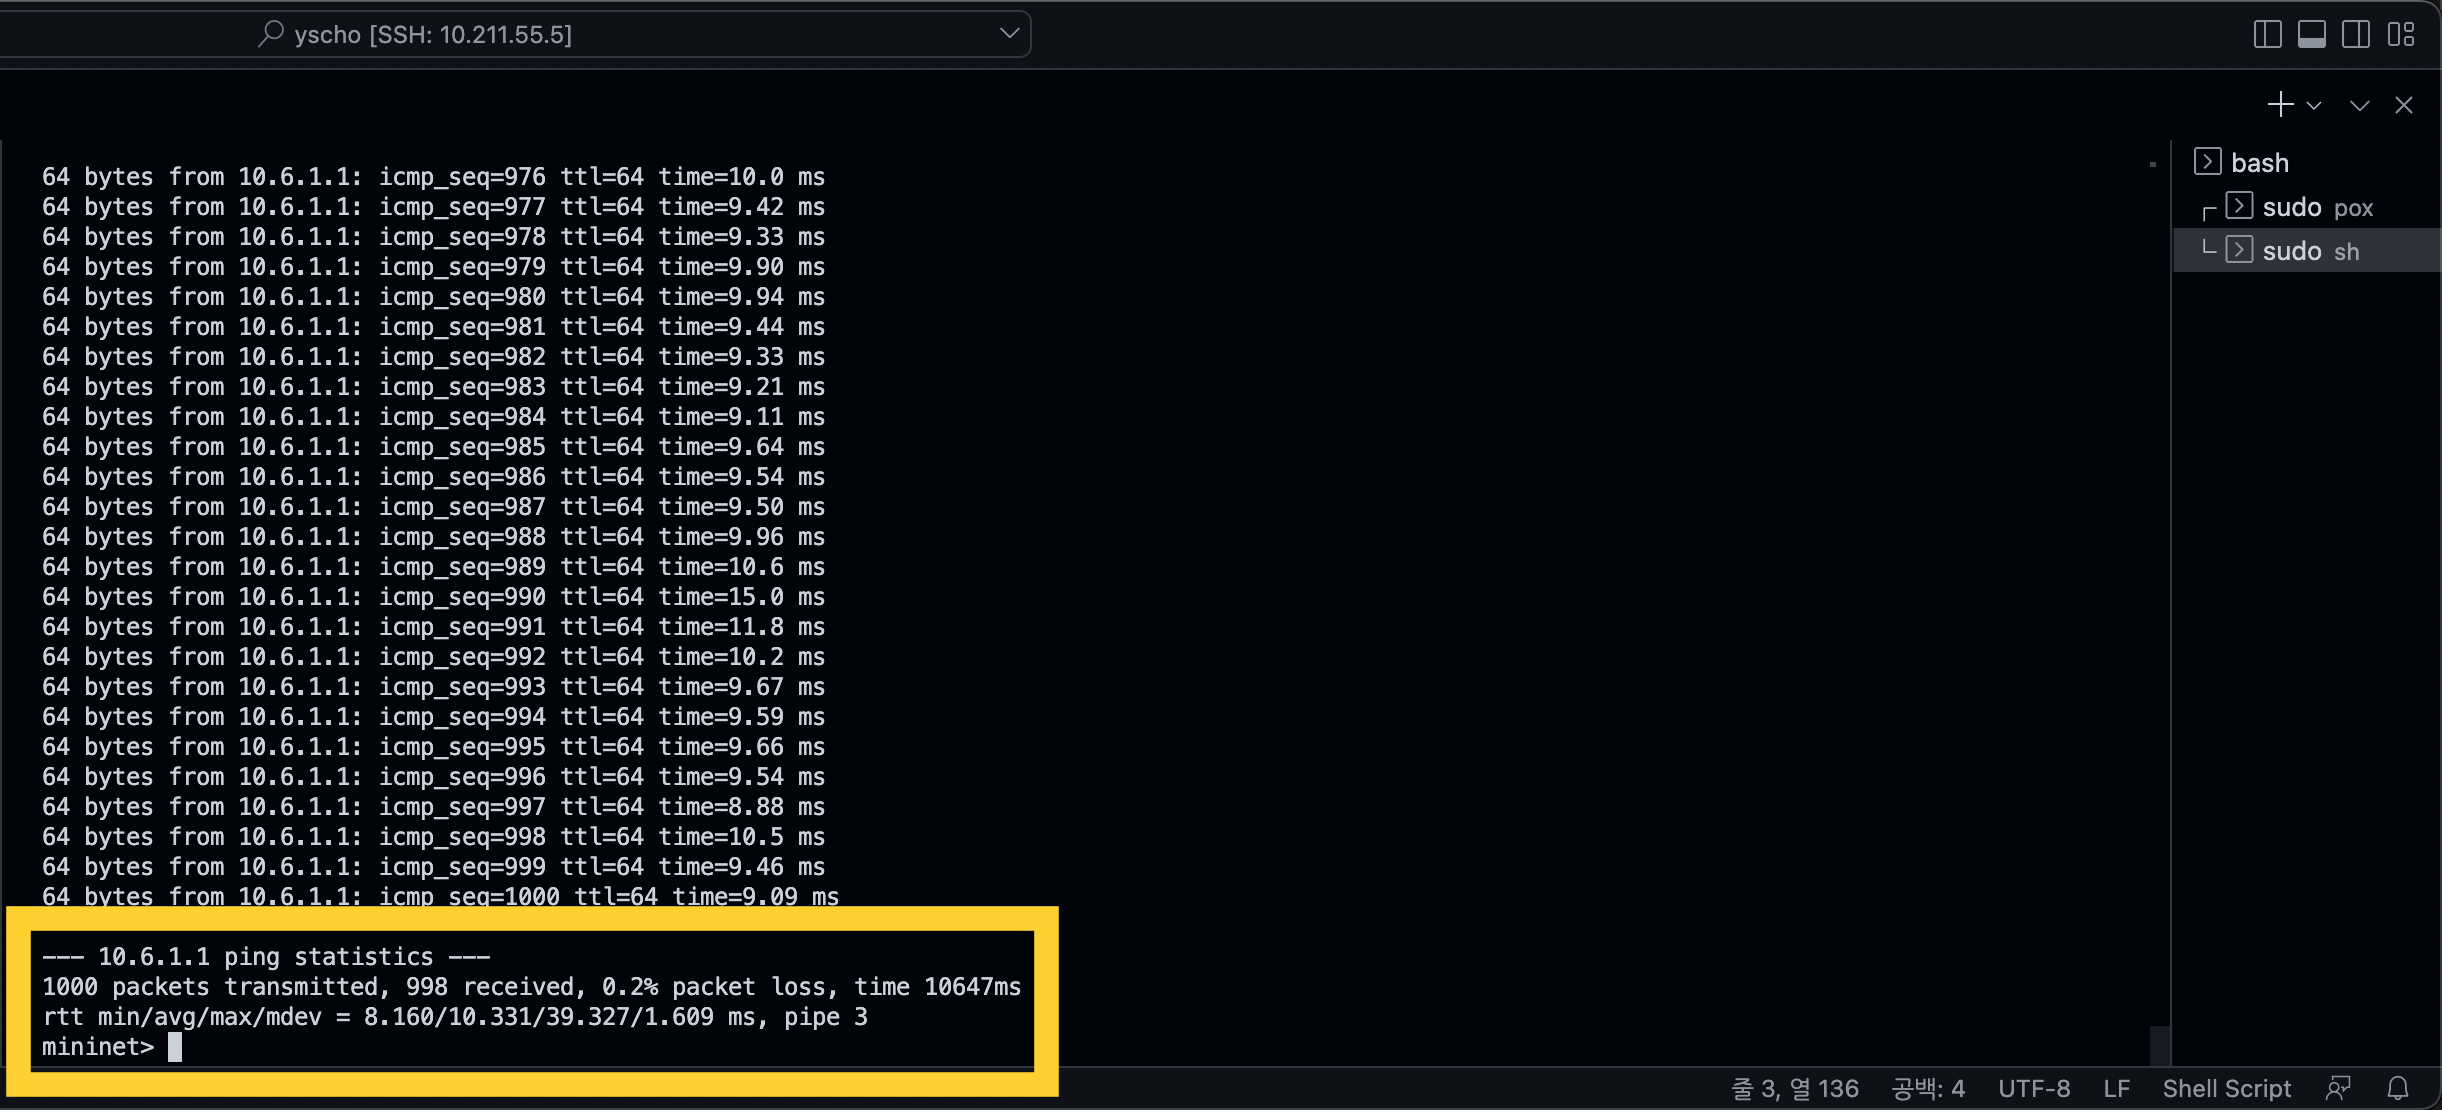
\includegraphics[width=.99\textwidth]{image/week08/3-2.png}
    	\caption{\footnotesize
    	  Experiment 3' pingtest results, $10.331\ ms$ average}
    	\vspace{-10pt}
    \end{figure}
    \clearpage
%---------------------------------------------------------------------------------%